\section{Introduction}
\thispagestyle{plain}
	\setcounter{page}{1}


This report is written as a bachelor project by computer science students at NTNU. The project revolves around upgrading and expanding features of a multi platform app called “Stedr” which is currently in beta. Stedr's purpose is to enable people to share their stories about places around the world. This can be anything from a famous attractions to just an ordinary building Trondheim. The contributors will be able to share stories and media through external services like Digitalt Fortalt, Flickr, Instagram and SoundCloud. With the application, users can view other peoples stories and images  to help them explore a certain place.

\subsection{The subject: IT2901}
\emph{IT2901: prosjektarbeid i informatikk} is the name of the course this project is a part of. Through this project the students will work in groups on a specific project within the scope of computer science. The institute will recommend tasks for the students to choose from. From here the students work self-reliantly under the supervision of employees at the institute. \textit{(Text based on the information gathered from the study guide.)}\\ The main purpose of the project is for the students to acquire practical experience with the software engineering process. Through working with a real customer in a the process, the students will gain valuable experience to prepare them for the working life.

\subsection{About Stedr}
The app “Stedr” was created in a collaboration between a group of Computer Science students from NTNU and Jacqueline Floch from SINTEF. 

Stedr is an app that connects places and stories. It combines the formal history with the social media experience. The latter will also help to create a network effect. 
We see Stedr as the first step towards a national effort for documenting narratives of places. Take the statue of Olav Tryggvason for instance. Here you can write a story about Olav, the building process, or something on the debate about removing it. That being said, Stedr is made to experience - not for creating content. To create a story takes time. It requires finding sources, put together materials, editing etc. This is not something that can be performed easily on a smartphone.

Ideally we wanted to create a social network for cultural heritage - a kind of GoGoBot for cultural heritage - but this is a much more extensive project. The question is also who would drive such a platform? Kulrurådet offers a platform called Digitalt Fortalt for stories. This is unprecedented and no other countries in Europe offers something like this. But unfortunately, Digitalt Fortalt has many limitations and it is a bit old fashioned. Europeana is an alternative that has support for user generated content and might thus be used in Stedr in the future.

The main goal of Stedr is to engage people more in the cultural heritage by
\begin{enumerate}
\item Giving them easy access to stories related to a cultural heritage. \item Providing different narratives for people who have different interests like history, art, sports, music etc. \item Utilizing network effects to increase awareness about places.
\end{enumerate}

Only about half of Europe's population visited a cultural venue in 2010. This is not a satisfying statistic and hopefully in time, Stedr will help to improve this by making people aware of interesting places. A place in Stedr is a point of culture heritage. All places have several stories associated with them. That means there is a potential for providing various stories from each place.

To this date, there is many books related to locations, buildings and art in Trondheim, but several of these books are no longer available in book stores. It is also very inconvenient to walk around with books all the time. Is not it amazing that we do not have access to all this information on the mobile in 2013? Documentation and dissemination of culture in the countryside is of course challenging. There are countless places, many of which lie outside the responsibility of institutions. Associations and individual enthusiasts have helped to gather information and document the places, but the results are fragmented.

So the first step with Stedr is to create a great cultural user experience. To provide the opportunity to discover new places. The second step would be to engage people to tell about places around them.

\clearpage

\subsection{Stakeholders}
In this subsection we will present the main people involved with the project. 

\subsubsection{The team}

\begin{figure}[!ht]
\begin{center}
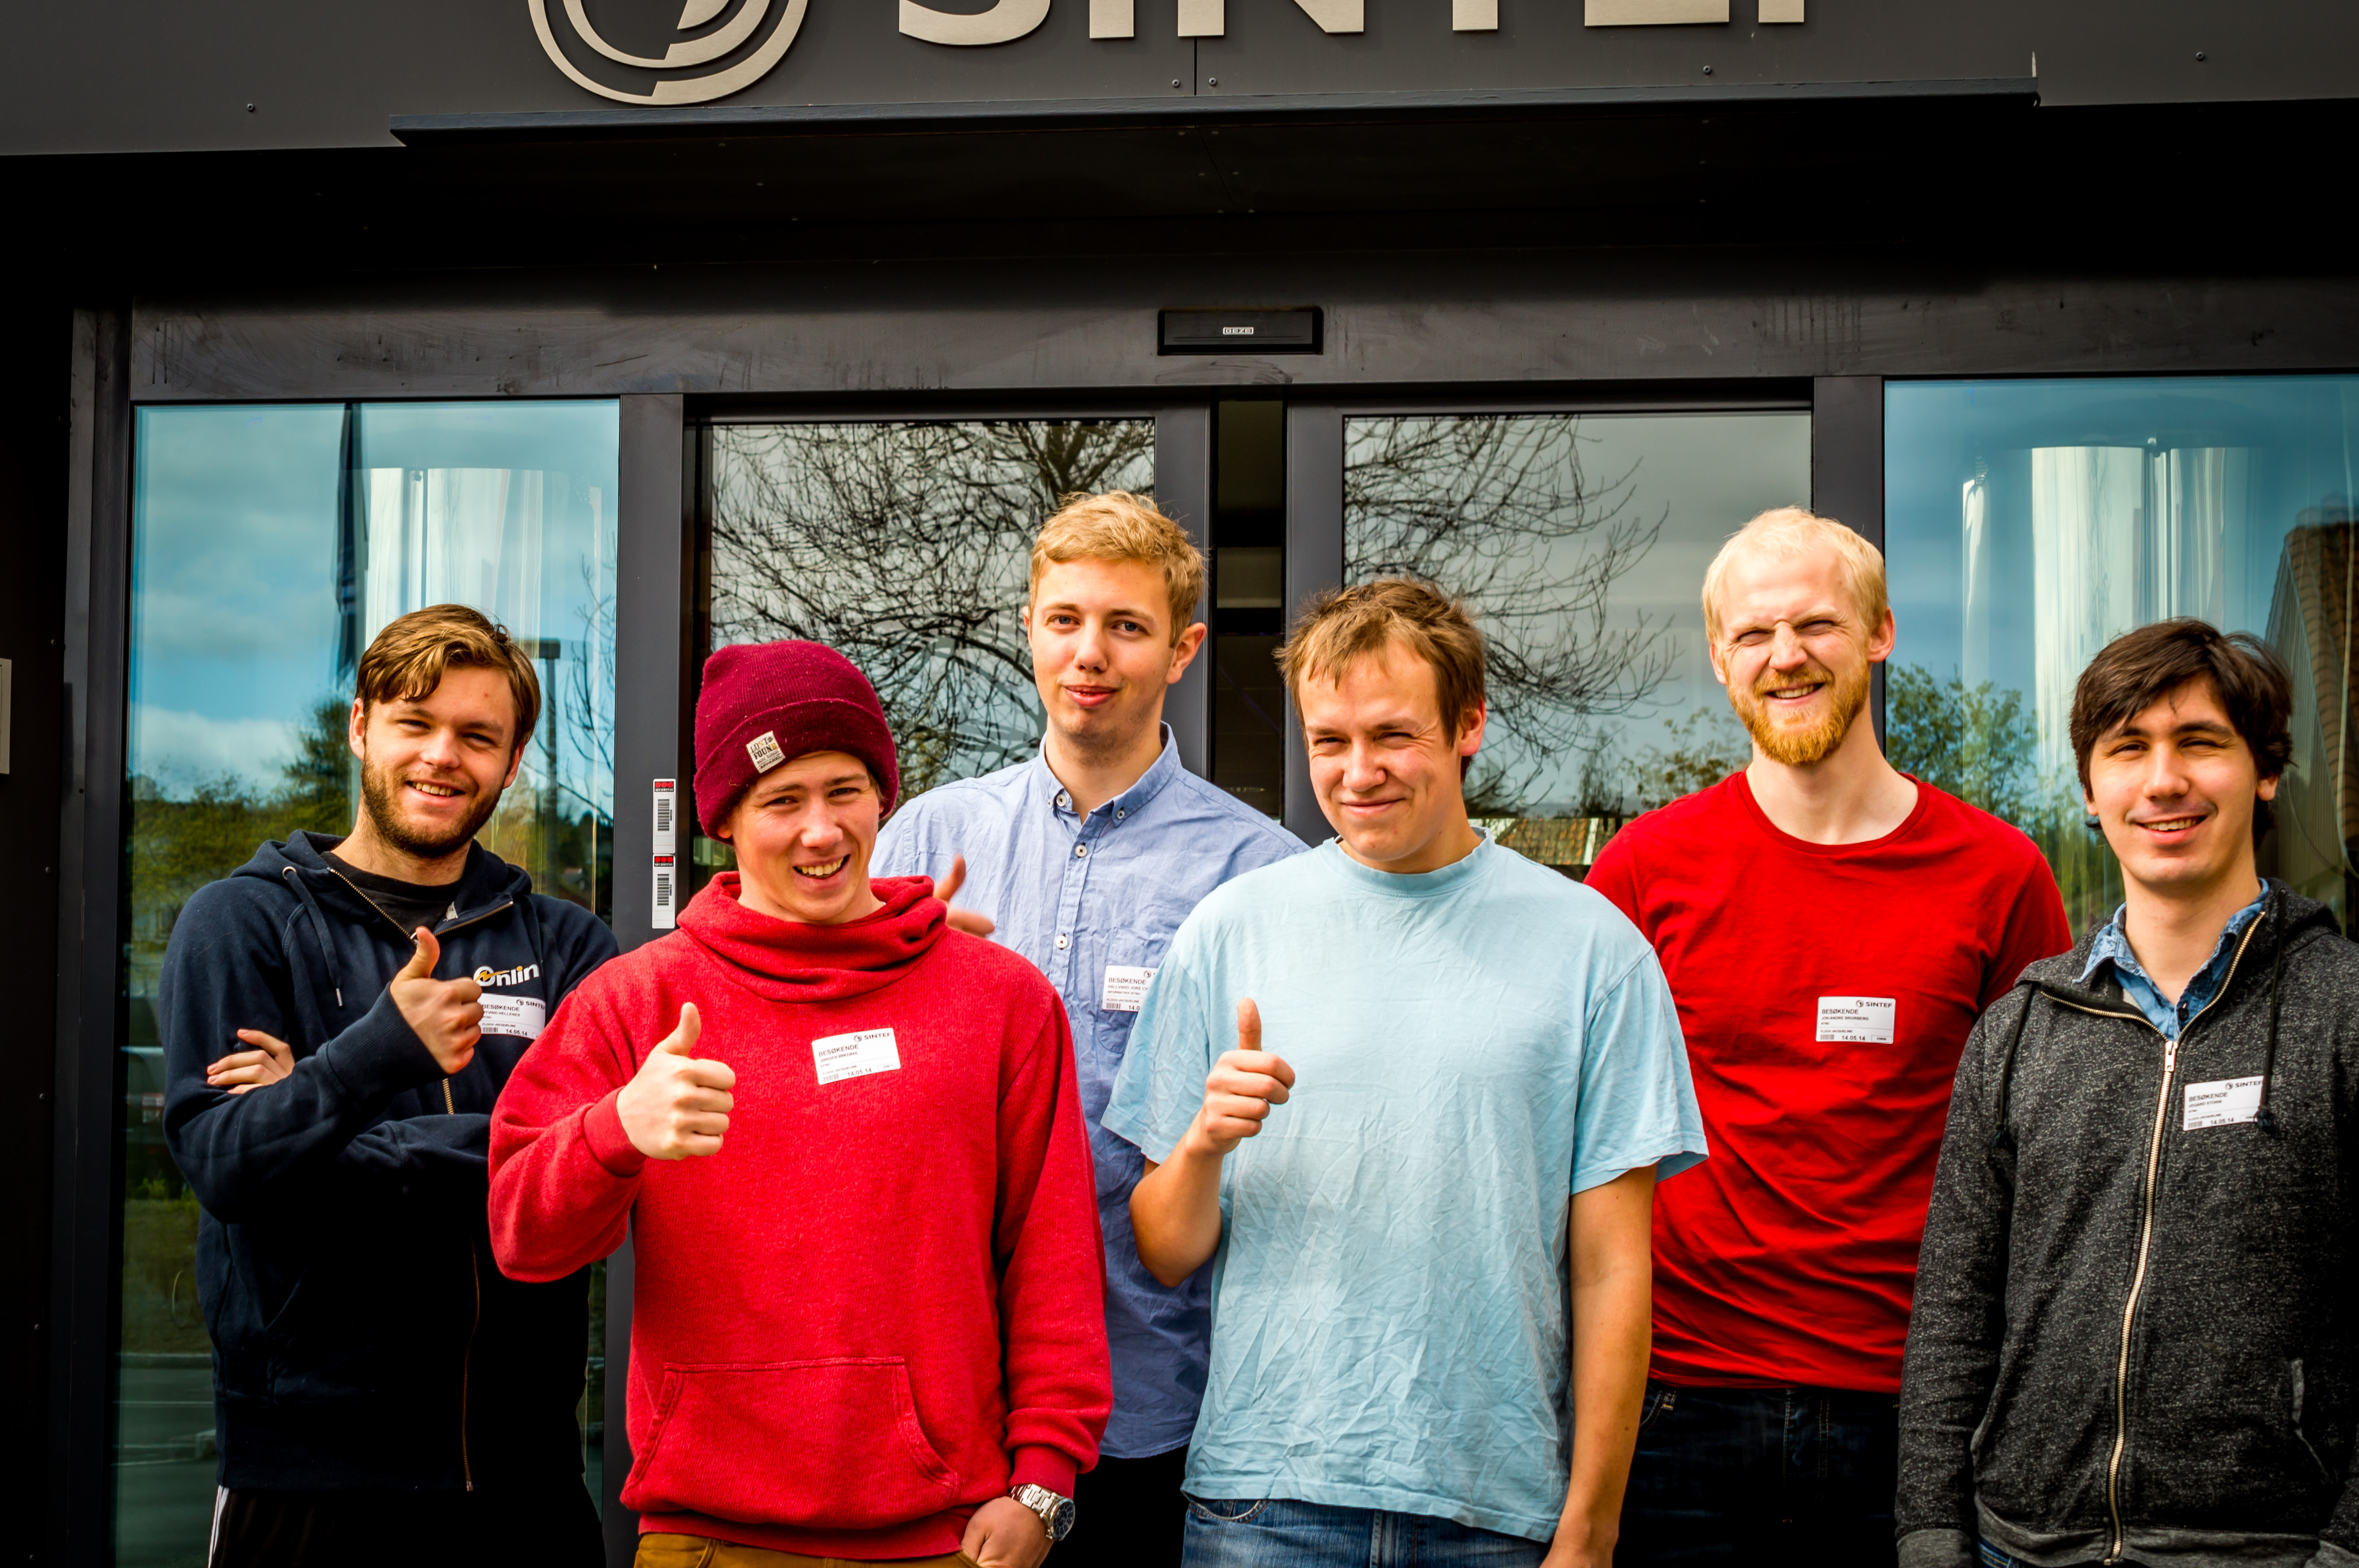
\includegraphics[width=0.7\textwidth]{res/theTeam.jpg}
\caption{The Group Members}
\end{center}
\end{figure}

The team consists of six students all taking a Bachelor degree in Informatics at The Norwegian University of Science and Technology (NTNU). In our group we have a great variation in areas of expertise and knowledge which helped us greatly during the course of the project. Having expertise in many different areas we could help each other and share knowledge across the group to make everybody suited to different tasks. The importance of this project made the whole group very motivated to work for a good result.
We are:

\begin{table}[!ht]
\begin{tabular}{r|p{11cm}}
\textbf{Hallvard Jore Christensen} & \texttt{hallvarc@stud.ntnu.no}\\[6pt]
\textbf{Jon-André Brurberg} & \texttt{jonandbr@stud.ntnu.no}\\[6pt]
\textbf{Jørgen Rugelsjøen Wikdahl} & \texttt{jorgenrw@stud.ntnu.no}\\[6pt]
\textbf{Tor Barstad} & \texttt{torob@stud.ntnu.no}\\[6pt]
\textbf{Vegard Storm} & \texttt{vegs@stud.ntnu.no}\\[6pt]
\textbf{Øyvind Hellenes} & \texttt{oyvihell@stud.ntnu.no}\\
\end{tabular}
\captionsetup{textformat=empty,labelformat=blank}
\caption[The Team]{}
\end{table}


\subsubsection{Customer}
Our customer is SINTEF (The Foundation for Scientific and Industrial Research). They are the largest independent research organisation in Scandinavia. The organisation was established at the Norwegian Institute of Technology (NTH) in Trondheim in 1950 and expanded rapidly in the following years.

\begin{table}[!ht]
\begin{tabular}{r|p{11cm}}
\textbf{Jaqueline Floch} & \emph{Project Manager}   \texttt{Jacqueline.Floch@sintef.no}\\[4pt]
& Our main contact at SINTEF and coordinator of the project from the customers side. She is also the primary driver for the app this project evolves around. \\[8pt]
\textbf{Babak Farshchian} & \emph{Interim Project Manager}   \texttt{Babak.Farshchian@sintef.no}\\[4pt]
& After some unfortunate events made Jacqueline unavailable in the very beginning, Babak took over for a period of time until Jacqueline could return as our main contact. \\
\end{tabular}
\captionsetup{textformat=empty,labelformat=blank}
\caption[Customer]{}
\end{table}

\subsubsection{Course Staff}

\begin{table}[!ht]
\begin{tabular}{r|p{11cm}}
\textbf{Mohsen Anvaari} & \emph{Supervisor}   \texttt{mohsena@idi.ntnu.no}\\[6pt]
& Supervises our group during the project, giving feedback and support. \\[8pt]
\textbf{Monica Divitini} & \emph{Course co-ordinator}   \texttt{divitini@idi.ntnu.no}\\[6pt]
& Is the course co-ordinator and in charge of the subject.\\
\end{tabular}
\captionsetup{textformat=empty,labelformat=blank}
\caption[Course Staff]{}
\end{table}

\clearpage
\subsection{Report Structure}

\textbf{Chapter 1}\\
 The introduction chapter. Presenting the course, project and the different people involved in the project.\\[15pt]
\textbf{Chapter 2}\\
Chapter describing the pre-study phase of the project. Since this project is based on an existing project with a prototype product, this phase was important for us. This process is documented in this chapter summing up all our research. \\[15pt]
\textbf{Chapter 3}\\
This chapter describes the basis of our project with the main focus on the projects' structure. This includes how both the group and the project have been organized.\\[15pt]
\textbf{Chapter 4}\\
This is the Software Requirements Specification (SRS) for the new version of ``Stedr'', and may be read both as a single chapter in this report or a stand-alone document. The SRS describes the behaviour of the system consisting of a detailed description with supplementation of diagrams and tables.\\[15pt]
\textbf{Chapter 5}\\
In this chapter we are presenting the system focusing on the architectural part.\\[15pt]
\textbf{Chapter 6}\\
Here you will be presented with the whole implementation process, containing all the sprint iterations.\\[15pt]
\textbf{Chapter 7}\\
This chapter focuses on the testing phase of the project. Acceptance-, case- and non-functional requirements testing are among what is on the agenda in this section.\\[15pt]
\textbf{Chapter 8}\\
A detailed evaluation of both planning, process and finally a conclusion. \\[15pt]
\textbf{Chapter 9}\\
Attachments.\\[15pt]
After theses chapters the appendices follows, containing other important documents and charts.

